\documentclass{article}%
\usepackage[T1]{fontenc}%
\usepackage[utf8]{inputenc}%
\usepackage{lmodern}%
\usepackage{textcomp}%
\usepackage{lastpage}%
\usepackage{geometry}%
\geometry{margin=0.7in}%
\usepackage{ragged2e}%
\usepackage{graphicx}%
\usepackage{fancyhdr}%
%
\fancypagestyle{header}{%
\renewcommand{\headrulewidth}{0pt}%
\renewcommand{\footrulewidth}{0pt}%
\fancyhead{%
}%
\fancyfoot{%
}%
\fancyhead[L]{%
Page date: %
\linebreak%
2023{-}02{-}04%
}%
\fancyhead[C]{%
Georgia Institute of Technology%
}%
\fancyhead[R]{%
Page \thepage\ of \pageref{LastPage}%
}%
}%
%
\begin{document}%
\normalsize%
\pagestyle{header}%
\begin{minipage}{\textwidth}%
\centering%
\begin{Large}%
\textbf{HW2: Problem 2}%
\end{Large}%
\linebreak%
\begin{large}%
\textbf{Ian Dover}%
\end{large}%
\end{minipage}%
\section{Convert Image to Greyscale}%
\label{sec:ConvertImagetoGreyscale}%
Image converted to greyscale:%


\begin{figure}[h!]%
\centering%
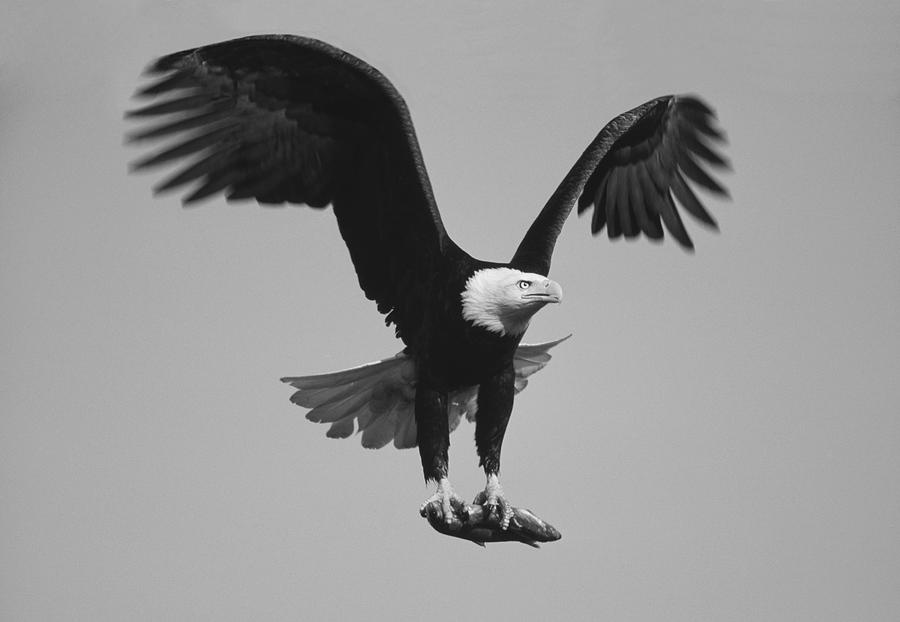
\includegraphics[width=120px]{/com.docker.devenvironments.code/reports/problem2/../../output/problem2/p2_Eagle_grayscale.jpg}%
\caption{Greyscale image.}%
\end{figure}

%
\section{Part 1}%
\label{sec:Part1}%
\subsection{Sobel Threshold: 10}%
\label{subsec:SobelThreshold10}%
Use the sobel operator on the image with a threshold of 10:%


\begin{figure}[h!]%
\centering%
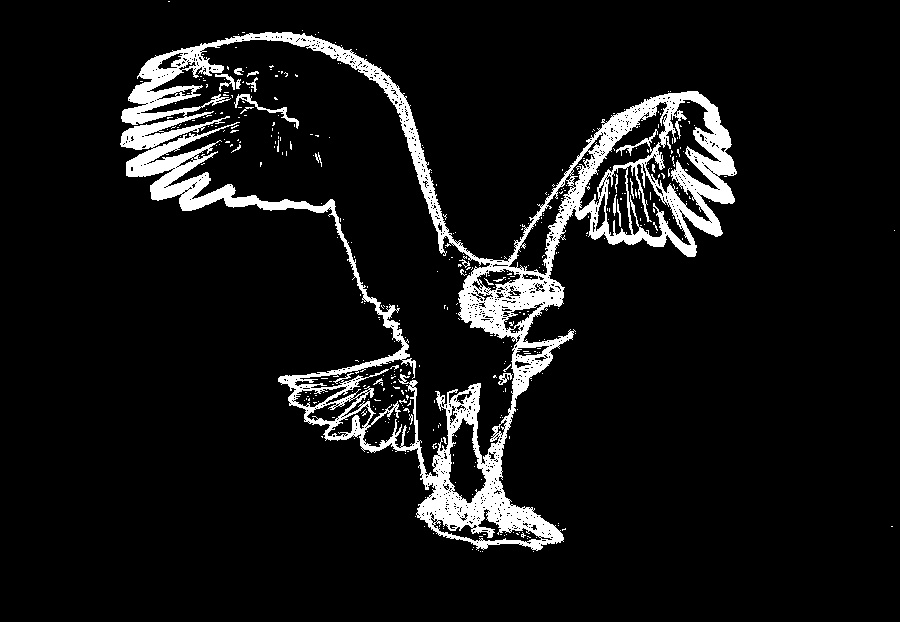
\includegraphics[width=120px]{/com.docker.devenvironments.code/reports/problem2/../../output/problem2/p2_part_1_sobel_thresh_10.jpg}%
\caption{Sobel threshold of 10.}%
\end{figure}

%
\subsection{Sobel Threshold: 50}%
\label{subsec:SobelThreshold50}%
Use the sobel operator on the image with a threshold of 50:%


\begin{figure}[h!]%
\centering%
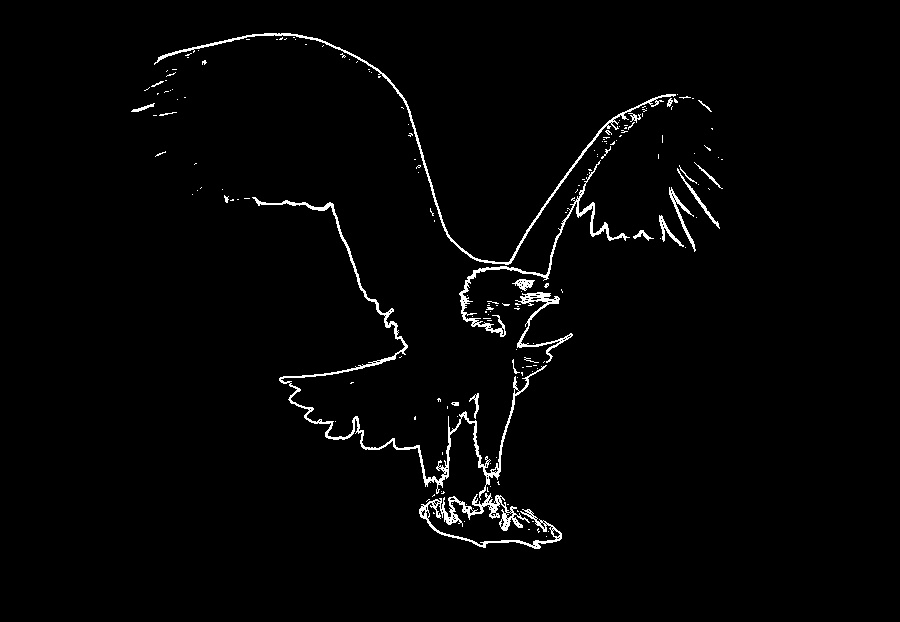
\includegraphics[width=120px]{/com.docker.devenvironments.code/reports/problem2/../../output/problem2/p2_part_1_sobel_thresh_50.jpg}%
\caption{Sobel threshold of 50.}%
\end{figure}

%
\newpage%
\subsection{Sobel Threshold: 100}%
\label{subsec:SobelThreshold100}%
Use the sobel operator on the image with a threshold of 100:%


\begin{figure}[h!]%
\centering%
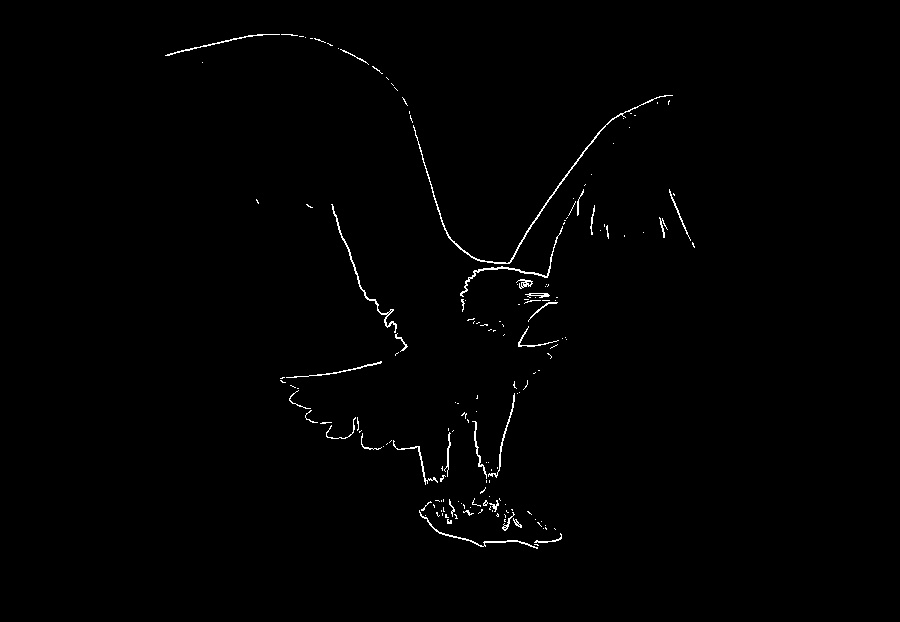
\includegraphics[width=120px]{/com.docker.devenvironments.code/reports/problem2/../../output/problem2/p2_part_1_sobel_thresh_100.jpg}%
\caption{Sobel threshold of 100.}%
\end{figure}

%
\subsection{Sobel Threshold: 150}%
\label{subsec:SobelThreshold150}%
Use the sobel operator on the image with a threshold of 150:%


\begin{figure}[h!]%
\centering%
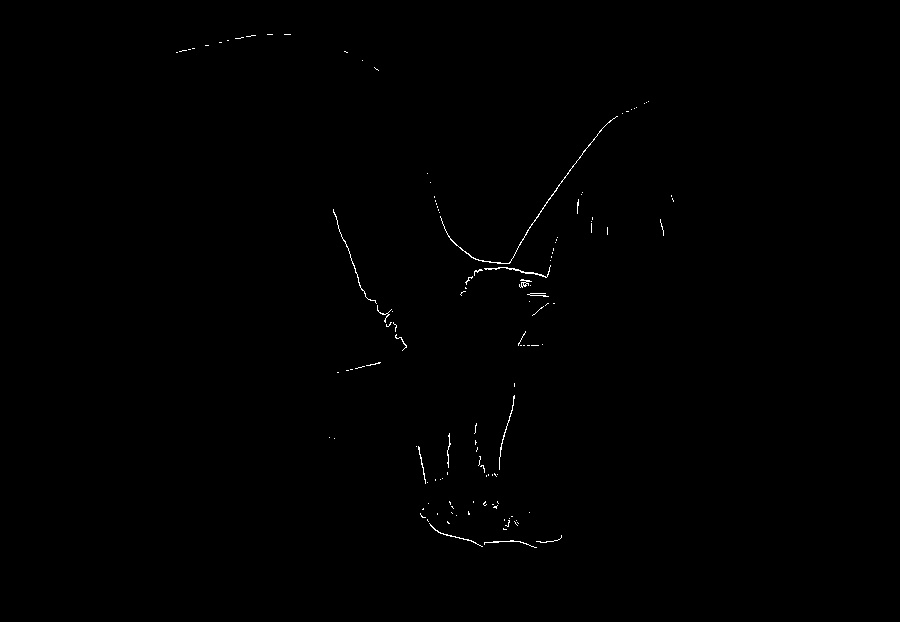
\includegraphics[width=120px]{/com.docker.devenvironments.code/reports/problem2/../../output/problem2/p2_part_1_sobel_thresh_150.jpg}%
\caption{Sobel threshold of 150.}%
\end{figure}

%
\subsection{Sobel Threshold: 200}%
\label{subsec:SobelThreshold200}%
Use the sobel operator on the image with a threshold of 200:%


\begin{figure}[h!]%
\centering%

\includegraphics[width=120px]{/com.docker.devenvironments.code/reports/problem2/../../output/problem2/p2_part_1_sobel_thresh_200.jpg}%
\caption{Sobel threshold of 200.}%
\end{figure}

%
\subsection{Sobel Threshold: 255}%
\label{subsec:SobelThreshold255}%
Use the sobel operator on the image with a threshold of 255:%


\begin{figure}[h!]%
\centering%

\includegraphics[width=120px]{/com.docker.devenvironments.code/reports/problem2/../../output/problem2/p2_part_1_sobel_thresh_255.jpg}%
\caption{Sobel threshold of 255.}%
\end{figure}

%
\newpage

%
\section{Part 2}%
\label{sec:Part2}%
\subsection{Prewitt Threshold: 10}%
\label{subsec:PrewittThreshold10}%
Use the prewitt operator on the image with a threshold of 10:%


\begin{figure}[h!]%
\centering%
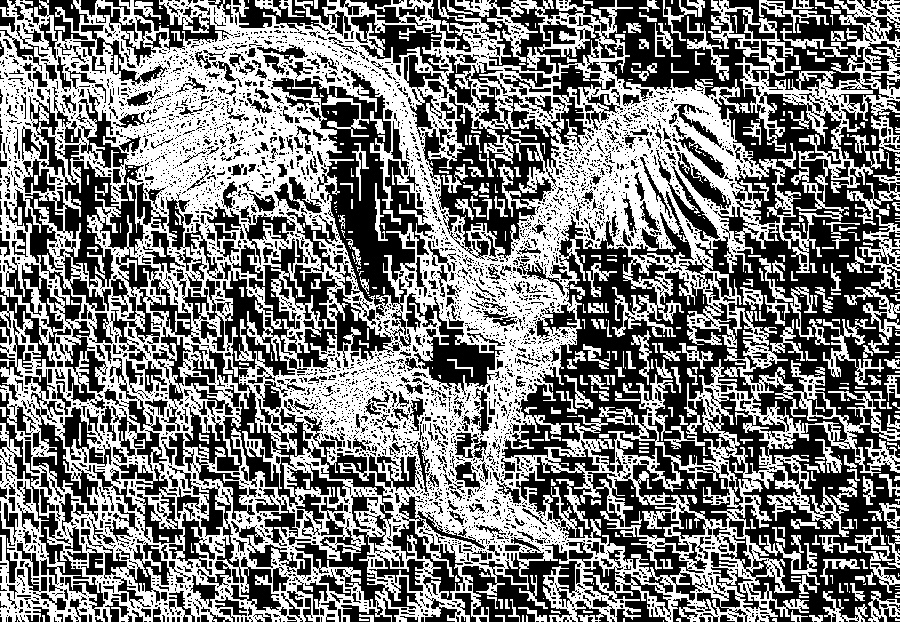
\includegraphics[width=120px]{/com.docker.devenvironments.code/reports/problem2/../../output/problem2/p2_part_2_prewitt_thresh_10.jpg}%
\caption{Prewitt threshold of 10.}%
\end{figure}

%
\subsection{Prewitt Threshold: 50}%
\label{subsec:PrewittThreshold50}%
Use the prewitt operator on the image with a threshold of 50:%


\begin{figure}[h!]%
\centering%
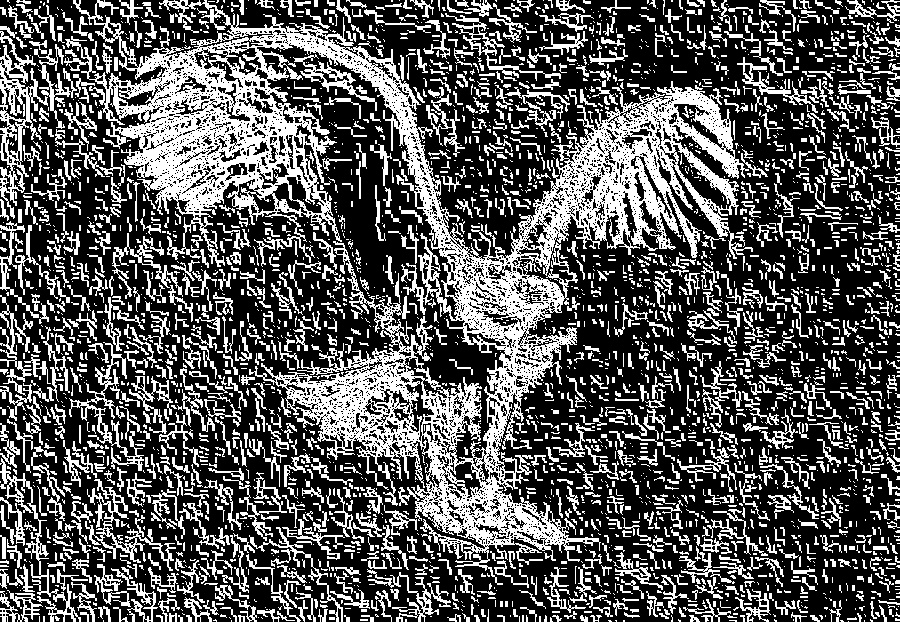
\includegraphics[width=120px]{/com.docker.devenvironments.code/reports/problem2/../../output/problem2/p2_part_2_prewitt_thresh_50.jpg}%
\caption{Prewitt threshold of 50.}%
\end{figure}

%
\newpage%
\subsection{Prewitt Threshold: 100}%
\label{subsec:PrewittThreshold100}%
Use the prewitt operator on the image with a threshold of 100:%


\begin{figure}[h!]%
\centering%
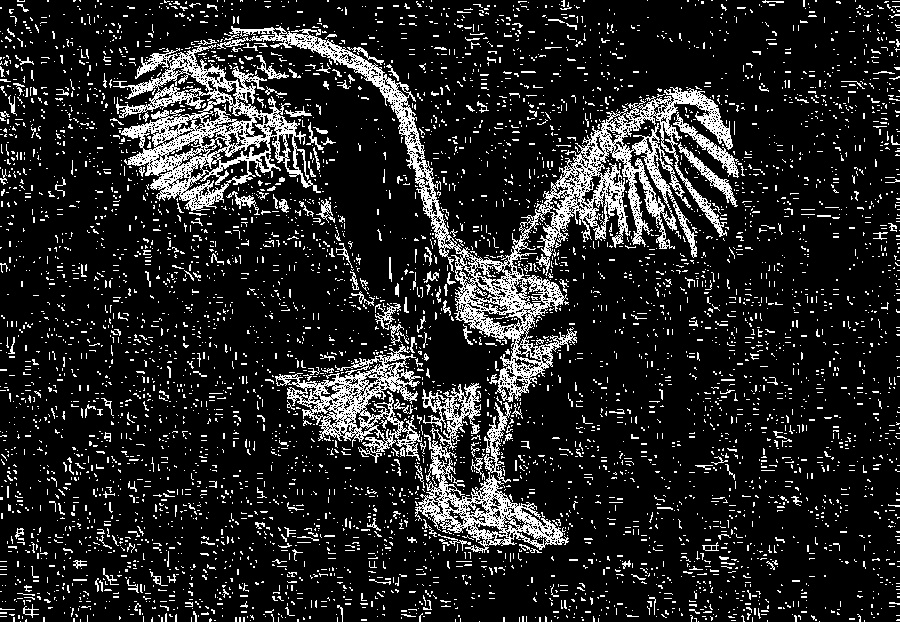
\includegraphics[width=120px]{/com.docker.devenvironments.code/reports/problem2/../../output/problem2/p2_part_2_prewitt_thresh_100.jpg}%
\caption{Prewitt threshold of 100.}%
\end{figure}

%
\subsection{Prewitt Threshold: 150}%
\label{subsec:PrewittThreshold150}%
Use the prewitt operator on the image with a threshold of 150:%


\begin{figure}[h!]%
\centering%
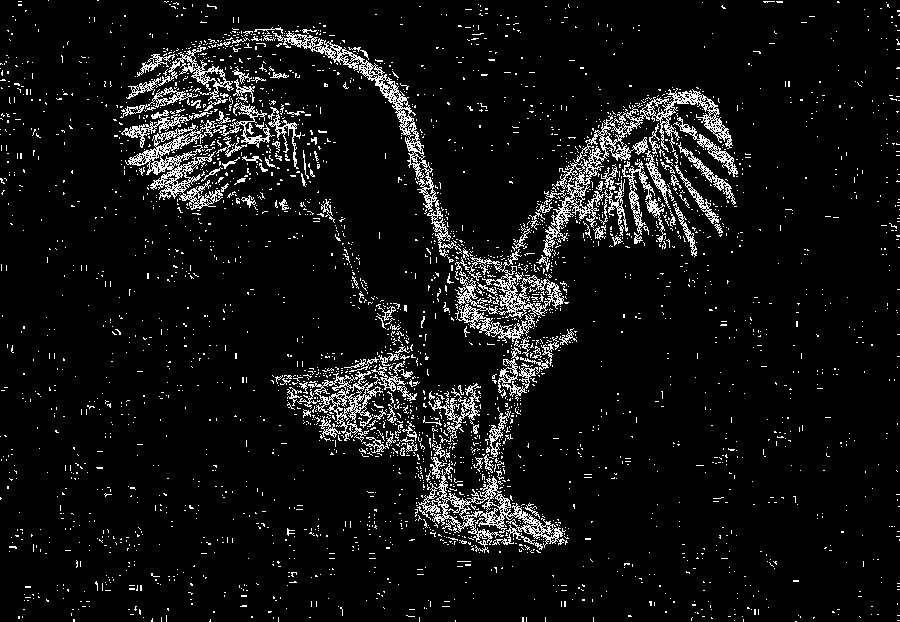
\includegraphics[width=120px]{/com.docker.devenvironments.code/reports/problem2/../../output/problem2/p2_part_2_prewitt_thresh_150.jpg}%
\caption{Prewitt threshold of 150.}%
\end{figure}

%
\subsection{Prewitt Threshold: 200}%
\label{subsec:PrewittThreshold200}%
Use the prewitt operator on the image with a threshold of 200:%


\begin{figure}[h!]%
\centering%
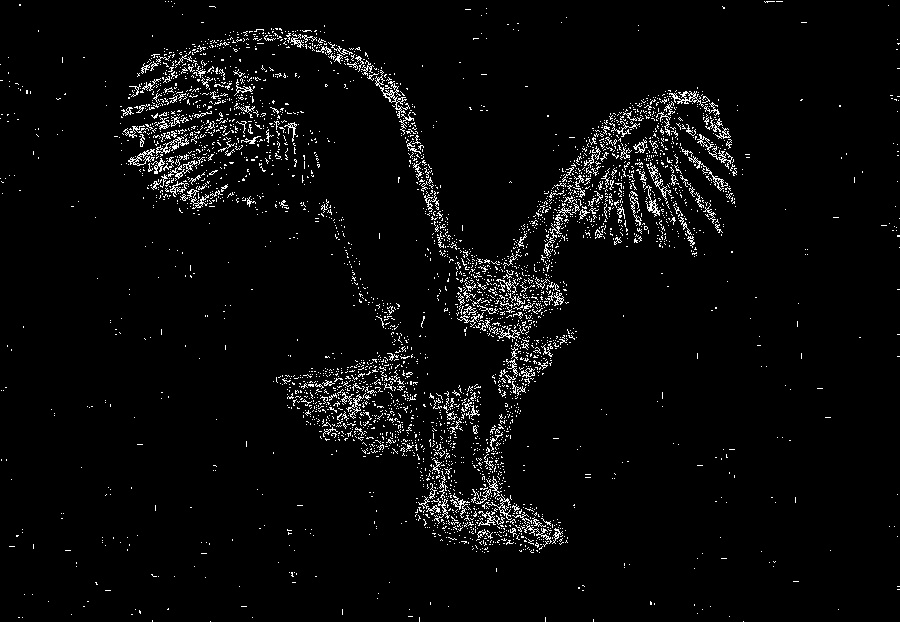
\includegraphics[width=120px]{/com.docker.devenvironments.code/reports/problem2/../../output/problem2/p2_part_2_prewitt_thresh_200.jpg}%
\caption{Prewitt threshold of 200.}%
\end{figure}

%
\subsection{Prewitt Threshold: 255}%
\label{subsec:PrewittThreshold255}%
Use the prewitt operator on the image with a threshold of 255:%


\begin{figure}[h!]%
\centering%

\includegraphics[width=120px]{/com.docker.devenvironments.code/reports/problem2/../../output/problem2/p2_part_2_prewitt_thresh_255.jpg}%
\caption{Prewitt threshold of 255.}%
\end{figure}

%
\newpage

%
\end{document}